% -*- coding: utf-8; -*-

\chapter{Plano de Ação}
\label{cha:Plano de Ação}

Antes de especificar o sistema e o algoritmo, foi realizada uma validação do problema. Alunos do Departamento de Informática da universidade foram entrevistados afim de descobrir quais dificuldades enfrentam durante o processo de matrícula e quais são as suas preferências ao montar uma grade disciplinar. O objetivo era identificar quais características de uma grade disciplinar contribuem para a satisfação do aluno e adicionar as funcionalidades necessárias no sistema e no algoritmo.

Com o problema validado, então o projeto passou por uma etapa de estudo anteriores. 
Foram estudados diferentes algoritmos de recomendação em contextos semelhantes ao sistema a ser desenvolvido, afim de se projetar o algoritmo que mais se adequa às necessidades do problema validado. 
Nessa etapa, também foram analisadas as fontes de informações disponibilizadas pela universidade e como cada fonte pode ser integrada no sistema. 

Após a etapa de estudos, deu-se início ao processe de modelagem dos requisitos, que foi seguido das elaborações de casos de usos, da arquitetura dos dados e da interface. 

Finalizada as elaborações e diagramas, o desenvolvimento foi iniciado, dando prioridade para o algoritmo. Depois de obter um algoritmo minimamente viável, foi desenvolvida a interface de planejamento para mostrar o funcionamento do algoritmo. 
Tanto o algoritmo com a interface foram desenvolvidas utilizando um modelo de desenvolvimento incremental, para que o sistema passasse por etapas de desenvolvimento, teste e validação com os alunos. 

A figura \ref{fig:fluxograma-acao} exemplifica o fluxo das etapas efetuadas, desde os estudos preliminares até os testes e trabalhos futuros.

\begin{figure}[ht]
    \begin{center}
    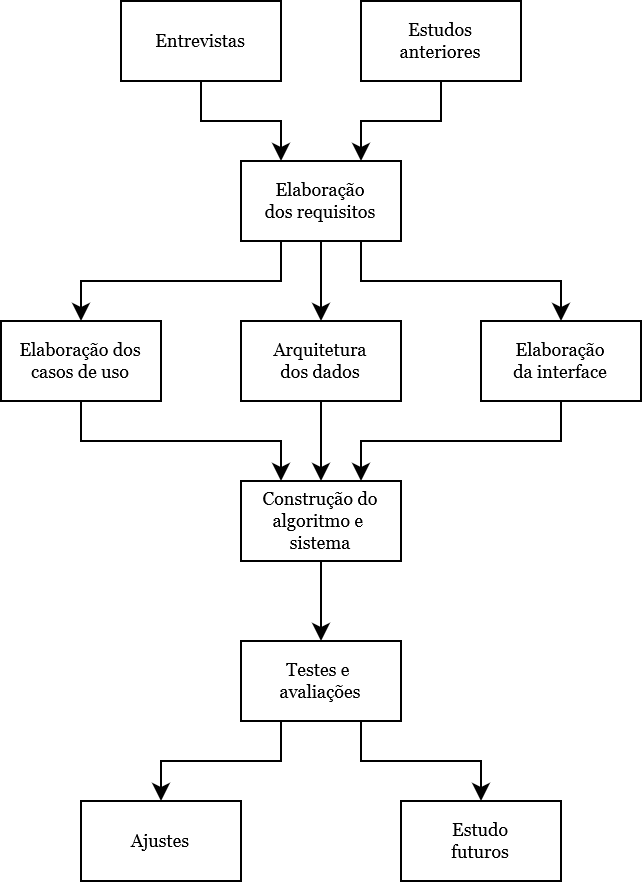
\includegraphics[width=260pt]{figuras/fluxograma-acao}
    \caption{Fluxo das etapas realizadas}
    \label{fig:fluxograma-acao}
    \end{center}
\end{figure}

\section{Cronograma original}

O cronograma inicial pode ser visualizado na figura \ref{fig:cronograma}.

\begin{figure}[ht]
    \begin{center}
    
\includegraphics[width=300pt]{figuras/cronograma}
    \caption{Cronograma original do projeto}
    \label{fig:cronograma}
    \end{center}
\end{figure}

\section{Cronograma real}

O cronograma real pode ser visualizado na figura \ref{fig:cronograma-atualizado}. Surgiu uma etapa de elaboração de especificações, que dizem respeito às elaborações de diagramas e tabelas de casos de uso, arquitetura de dados e interface, criadas antes da etapa de desenolvimento. O desenvolvimento teve seu tempo encurtado de forma extrema, pois elaborar as especificações tomou grande parte do tempo de desenvolvimento, mas mesmo com metade do tempo original foi possível implementar todas as funcionalidades planejadas.


\begin{figure}[ht]
    \begin{center}
    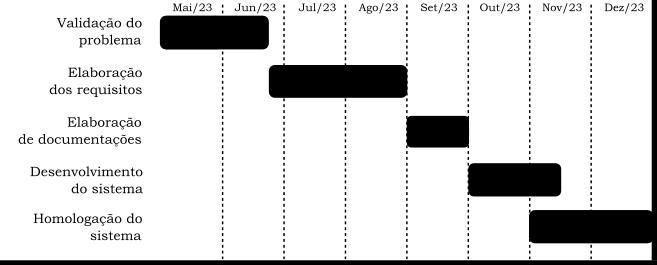
\includegraphics[width=300pt]{figuras/cronograma-atualizado}
    \caption{Cronograma atualizado do projeto}
    \label{fig:cronograma-atualizado}
    \end{center}
\end{figure}

